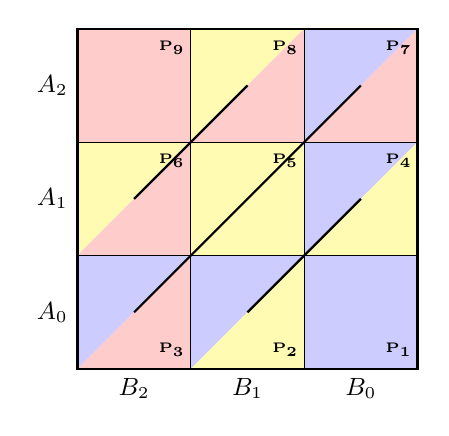
\begin{tikzpicture}[scale=1.2]
    % Define grid spacing
    \def\cellsize{1.2}
    
    % P9: A_2 B_2 (top-left)
    \draw[fill=red!20] (-2.4, 1.2) rectangle (-1.2, 2.4);
    \node[font=\tiny, black] at (-1.4, 2.2) {$\mathbf{P_9}$};
    
    % P8: A_2 B_1 (top-middle) - diagonal split with P6 using P5 and P9 colors
    \fill[yellow!30] (-1.2, 1.2) -- (-1.2, 2.4) -- (0, 2.4) -- cycle;
    \fill[red!20] (-1.2, 1.2) -- (0, 1.2) -- (0, 2.4) -- cycle;
    \draw (-1.2, 1.2) rectangle (0, 2.4);
    \node[font=\tiny, black] at (-0.2, 2.2) {$\mathbf{P_8}$};
    
    % P7: A_2 B_0 (top-right) - diagonal split with P3 using P1 and P9 colors
    \fill[blue!20] (0, 1.2) -- (0, 2.4) -- (1.2, 2.4) -- cycle;
    \fill[red!20] (0, 1.2) -- (1.2, 1.2) -- (1.2, 2.4) -- cycle;
    \draw (0, 1.2) rectangle (1.2, 2.4);
    \node[font=\tiny, black] at (1.0, 2.2) {$\mathbf{P_7}$};
    
    % P6: A_1 B_2 (middle-left) - diagonal split with P8 using P5 and P9 colors
    \fill[yellow!30] (-2.4, 0) -- (-2.4, 1.2) -- (-1.2, 1.2) -- cycle;
    \fill[red!20] (-2.4, 0) -- (-1.2, 0) -- (-1.2, 1.2) -- cycle;
    \draw (-2.4, 0) rectangle (-1.2, 1.2);
    \node[font=\tiny, black] at (-1.4, 1.0) {$\mathbf{P_6}$};
    
    % P5: A_1 B_1 (middle-middle)
    \draw[fill=yellow!30] (-1.2, 0) rectangle (0, 1.2);
    \node[font=\tiny, black] at (-0.2, 1.0) {$\mathbf{P_5}$};
    
    % P4: A_1 B_0 (middle-right) - diagonal split with P2 using P1 and P5 colors
    \fill[blue!20] (0, 0) -- (0, 1.2) -- (1.2, 1.2) -- cycle;
    \fill[yellow!30] (0, 0) -- (1.2, 0) -- (1.2, 1.2) -- cycle;
    \draw (0, 0) rectangle (1.2, 1.2);
    \node[font=\tiny, black] at (1.0, 1.0) {$\mathbf{P_4}$};
    
    % P3: A_0 B_2 (bottom-left) - diagonal split with P7 using P1 and P9 colors
    \fill[blue!20] (-2.4, -1.2) -- (-2.4, 0) -- (-1.2, 0) -- cycle;
    \fill[red!20] (-2.4, -1.2) -- (-1.2, -1.2) -- (-1.2, 0) -- cycle;
    \draw (-2.4, -1.2) rectangle (-1.2, 0);
    \node[font=\tiny, black] at (-1.4, -1.0) {$\mathbf{P_3}$};
    
    % P2: A_0 B_1 (bottom-middle) - diagonal split with P4 using P1 and P5 colors
    \fill[blue!20] (-1.2, -1.2) -- (-1.2, 0) -- (0, 0) -- cycle;
    \fill[yellow!30] (-1.2, -1.2) -- (0, -1.2) -- (0, 0) -- cycle;
    \draw (-1.2, -1.2) rectangle (0, 0);
    \node[font=\tiny, black] at (-0.2, -1.0) {$\mathbf{P_2}$};
    
    % P1: A_0 B_0 (bottom-right)
    \draw[fill=blue!20] (0, -1.2) rectangle (1.2, 0);
    \node[font=\tiny, black] at (1.0, -1.0) {$\mathbf{P_1}$};
    
    % Lines connecting symmetric elements
    % P8 (A_2 B_1) and P6 (A_1 B_2)
    \draw[black, thick] (-0.6, 1.8) -- (-1.8, 0.6);
    
    % P7 (A_2 B_0) and P3 (A_0 B_2)
    \draw[black, thick] (0.6, 1.8) -- (-1.8, -0.6);
    
    % P4 (A_1 B_0) and P2 (A_0 B_1)
    \draw[black, thick] (0.6, 0.6) -- (-0.6, -0.6);
    
    % Outer border
    \draw[thick] (-2.4, -1.2) rectangle (1.2, 2.4);
    
    % Labels for inputs
    % Vertical axis (A) - left side
    \node[left, font=\small] at (-2.4, 1.8) {$A_2$};
    \node[left, font=\small] at (-2.4, 0.6) {$A_1$};
    \node[left, font=\small] at (-2.4, -0.6) {$A_0$};
    
    % Horizontal axis (B) - bottom
    \node[below, font=\small] at (-1.8, -1.2) {$B_2$};
    \node[below, font=\small] at (-0.6, -1.2) {$B_1$};
    \node[below, font=\small] at (0.6, -1.2) {$B_0$};
\end{tikzpicture}
